%% Time-stamp: <2018-10-18 20:24:12 (marc)>
\documentclass[xcolor=x11names,compress,mathserif]{beamer}

\newcommand{\hackspace}{\hspace{4.2mm}}
\newcommand{\showstudent}[1]{}
\newcommand\hmmax{0}
\newcommand\bmmax{0}



% talk/author information
\newcommand{\authorname}{Yingzhen Li}
\newcommand{\authoremail}{yingzhen.li@imperial.ac.uk}
\newcommand{\authoraffiliation}{
  Department of Computing\\Imperial
  College London}
\newcommand{\authortwitter}{liyzhen2}
\newcommand{\slidesettitle}{\imperialBlue{Gradient Descent Convergence}}
\newcommand{\footertitle}{Gradient Descent Convergence}
\newcommand{\location}{Imperial College London}
\newcommand{\talkDate}{October 24, 2022}



\date{\imperialGray{\talkDate}}



% load defaults
%\usepackage{../MarkMathCmds}
\selectcolormodel{rgb}
\usepackage{ifxetex,ifluatex}
\newif\ifxetexorluatex
\ifxetex
  \xetexorluatextrue
\else
  \ifluatex
    \xetexorluatextrue
  \else
    \xetexorluatexfalse
  \fi
\fi

\usepackage{textpos}
%\usepackage{arabtex}
\usepackage{tikz}
\usetikzlibrary{decorations.markings}
\usetikzlibrary{arrows}
\usetikzlibrary{shapes}
\usetikzlibrary{plotmarks}
\usetikzlibrary{mindmap,trees,backgrounds}

\tikzstyle{every picture}+=[remember picture]

%\usepackage{movie15}
% \usepackage{pdfpages}
%\usepackage{xmpmulti}

\usepackage{anyfontsize}
\usepackage{wrapfig}
\usepackage{animate}
\usepackage{multirow}
\usepackage{multimedia}
\usepackage{xmpmulti}
%\usepackage[latin9]{inputenc}
\usepackage[english]{babel}
\usepackage{scalefnt}
\usepackage{verbatim}
\usepackage{url}
% \usepackage{pgf,pgfarrows,pgfnodes}
\usepackage{textpos}
\usepackage[tight,ugly]{units}
\usepackage{url}
\usepackage{bbm}
\usepackage[english]{babel}
\usepackage{fancyhdr}
\usepackage{bm} % correct bold symbols, like \bm
\usepackage{amsmath}
\usepackage{amsfonts}
\usepackage{amssymb}
\usepackage{mathrsfs}
\usepackage{mathtools}
\usepackage{color}
\usepackage{cancel}
\usepackage{algorithm}
\usepackage{algpseudocode}
\usepackage{mathrsfs}
\usepackage{listings}
\usepackage{graphicx} % for pdf, bitmapped graphics files
\usepackage{mathtools}
\usepackage{units}
\usepackage{subfig}
\usepackage{enumerate}
\usepackage[comma,authoryear]{natbib}
\usepackage{dsfont}


\ifxetexorluatex
\usepackage{fontspec}
\setmainfont[Scale=0.8]{OpenDyslexic-Regular}
\else
\usefonttheme{professionalfonts}
\fi

\renewcommand{\vec}[1]{{\boldsymbol{{#1}}}} % vector
\newcommand{\mat}[1]{{\boldsymbol{{#1}}}} % matrix
% \newcommand{\KL}[2]{\mathrm{KL}(#1\|#2)} % KL divergence
\newcommand{\R}[0]{\mathds{R}} % real numbers
\newcommand{\Z}[0]{\mathds{Z}} % integers
\newcommand{\tr}[0]{\text{tr}} % trace
% \newcommand{\inv}{^{-1}}
% \DeclareMathOperator*{\diag}{diag}
\newcommand{\E}{\mathds{E}} % expectation
\newcommand{\var}{\mathds{V}}
\newcommand{\gauss}[2]{\mathcal{N}\big(#1,\,#2\big)}
\newcommand{\gaussx}[3]{\mathcal{N}\big(#1\,|\,#2,\,#3\big)}
\newcommand{\gaussBig}[2]{\mathcal{N}\left(#1,\,#2\right)}
\newcommand{\gaussxBig}[3]{\mathcal{N}\left(#1\,\left|\,#2,\,#3\right.\right)}
\newcommand{\Ber}[0]{\mathrm{Ber}} % Bernoulli distribution
\DeclareMathOperator{\cov}{Cov}
\ifxetexorluatex
\renewcommand{\T}[0]{^\top}
\renewcommand{\d}[0]{\text{d}} % derivative
\else
\newcommand{\T}[0]{^\top}
\renewcommand{\d}[0]{\text{d}} % derivative
\fi
% calculus
\newcommand{\pdiff}[1]{\frac{\partial}{\partial #1}}
\newcommand{\pdiffF}[2]{\frac{\partial #1}{\partial #2}}
\newcommand{\diffF}[2]{\frac{{\d}#1}{{\d}#2}}
\newcommand{\diffFII}[2]{\frac{{\d}^2 #1}{{\d}#2^2}}
\newcommand{\diff}[1]{\frac{{\d}}{{\d}#1}}
\newcommand{\diffII}[1]{\frac{{\d}^2}{{\d}#1^2}}
\newcommand{\class}[0]{\mathcal{C}}

\newcommand{\idx}[1]{{(#1)}}
% \newcommand{\norm}[1]{\left\|#1\right\|}
\newcommand{\proj}[1]{\tilde{#1}}
\newcommand{\pcacoord}{z}
\newcommand{\pcacoordnew}{\zeta}
\newcommand{\latent}{z}
% \newcommand{\given}{\,|\,}
\newcommand{\genset}[1]{\mathrm{span}[#1]} % generating set
\newcommand{\set}[1]{\mathcal{#1}} % set
\newcommand{\fixgmfont}[1]{\scalebox{0.8}{#1}}



\usepackage{pifont}% http://ctan.org/pkg/pifont
\newcommand{\cmark}{{\color{green!40!black}\ding{51}}}%
\newcommand{\xmark}{{\color{red}\ding{55}}}%
\newcommand{\green}[1]{{\bf{\textcolor{green}{#1}}}}
\newcommand{\red}[1]{{\bf{\textcolor{red}{#1}}}}

\newcommand<>\red[1]{{\color#2[rgb]{1,0,0}#1}}
\newcommand<>\blue[1]{{\color#2[rgb]{0,0,1}#1}}
\newcommand<>\yellow[1]{{\color#2{camyellow}#1}}
\newcommand<>\green[1]{{\color#2[rgb]{0,0.6,0.0}#1}}
\newcommand<>\violet[1]{{\color#2[rgb]{0.6,0,0.6}#1}}
\newcommand<>\orange[1]{{\color#2[rgb]{1,0.5,0}#1}}
\newcommand<>\black[1]{{\color#2[rgb]{0,0,0}#1}}
\newcommand<>\steel[1]{{\color#2[rgb]{0,0,0.8}#1}}
\newcommand<>\darkblue[1]{{\color#2[rgb]{0,0,0.6}#1}}
\newcommand<>\lightblue[1]{{\color#2[rgb]{0.4,0.4,0.7}#1}}
\newcommand<>\gray[1]{{\color#2[rgb]{0.4,0.4,0.4}#1}}
\newcommand<>\greenish[1]{{\color#2[rgb]{0.45, 0.66, 0.45}#1}}
\newcommand<>\redish[1]{{\color#2[rgb]{0.7843    0.3706    0.3706}#1}}
\definecolor{redishTIKZ}{rgb}{0.7843, 0.3706, 0.3706}
\definecolor{imperialBlue}{rgb}{0.058, 0.219, 0.418}
\definecolor{aimsbrown}{rgb}{0.539, 0.117, 0.015}
% \definecolor{imperialGray}{rgb}{0.414, 0.488, 0.671 }
\definecolor{imperialGray}{RGB}{109,153, 204}
\definecolor{aimslightbrown}{RGB}{138,88,84}
\newcommand<>\imperialBlue[1]{{\color#2[rgb]{0.058, 0.219, 0.418}#1}}
\newcommand<>\aimsbrown[1]{{\color#2[rgb]{0.539, 0.117, 0.015}#1}}
%\newcommand<>\imperialGray[1]{{\color#2[rgb]{0.414, 0.488, 0.671}#1}}
\newcommand<>\imperialGray[1]{{\color#2[RGB]{109,153, 204}#1}}
\newcommand<>\aimslightbrown[1]{{\color#2[RGB]{138,88,84}#1}}
\newcommand<>\lightgray[1]{{\color#2[rgb]{0.8,0.8,0.8}#1}}
%\newcommand<>\highlightcolor[1]{{\color#2[rgb]{0,0,1}#1}}
\newcommand{\highlight}[1]{{\bf\steel{#1}}}
%\newcommand{\newblock}[0]{}

%\newcommand{\arrow}[0]{\includegraphics[height=5pt]{./figures/arrow}\hspace{3pt}}

\renewcommand{\emph}[1]{\textbf{\steel{{#1}}}}

\renewcommand{\alert}[1]{{\bf\red{{#1}}}}

\newcommand{\arrow}{
\begin{tikzpicture}
\draw [black!40!green, fill=black!40!green] (0,-0.12) -- (0,0.12) --
(0.15,0);
\draw [black!40!green, fill=black!40!green] (0.15,-0.12) -- (0.15,0.12) --
(0.3,0); 
\end{tikzpicture}
}

\geometry{left=0.45cm,top=0cm,right=0.45cm}


\newcommand{\logoimagepath}{./figures/imperial}
\newcommand{\highlightcolor}{blue!80!black}
%\newcommand{\headbarcolor}{imperialBlue}
\newcommand{\headbarcolor}{imperialBlue}
\institute{}

\newcommand{\coursetitle}{}

\newcommand{\slidesetsubtitle}{}
\newcommand{\slidesetnumber}{01}
\usefonttheme{professionalfonts}


\usetikzlibrary{decorations.fractals}
% tikzlibrary.code.tex
%
% Copyright 2010-2011 by Laura Dietz
% Copyright 2012 by Jaakko Luttinen
%
% The MIT License
%
% See LICENSE file for more details.

% Load other libraries
\usetikzlibrary{shapes}
\usetikzlibrary{fit}
\usetikzlibrary{chains}
\usetikzlibrary{arrows}

% Latent node
\tikzstyle{latent} = [circle,fill=white,draw=black,inner sep=1pt,
minimum size=20pt, font=\fontsize{10}{10}\selectfont, node distance=1]
% Observed node
\tikzstyle{obs} = [latent,fill=gray!25]
% Constant node
\tikzstyle{const} = [rectangle, inner sep=0pt, node distance=1]
% Factor node
\tikzstyle{factor} = [rectangle, fill=black,minimum size=5pt, inner
sep=0pt, node distance=0.4]
% Deterministic node
\tikzstyle{det} = [latent, diamond]

% Plate node
\tikzstyle{plate} = [draw, rectangle, rounded corners, fit=#1]
% Invisible wrapper node
\tikzstyle{wrap} = [inner sep=0pt, fit=#1]
% Gate
\tikzstyle{gate} = [draw, rectangle, dashed, fit=#1]

% Caption node
\tikzstyle{caption} = [font=\footnotesize, node distance=0] %
\tikzstyle{plate caption} = [caption, node distance=0, inner sep=0pt,
below left=5pt and 0pt of #1.south east] %
\tikzstyle{factor caption} = [caption] %
\tikzstyle{every label} += [caption] %

%\pgfdeclarelayer{b}
%\pgfdeclarelayer{f}
%\pgfsetlayers{b,main,f}

% \factoredge [options] {inputs} {factors} {outputs}
\newcommand{\factoredge}[4][]{ %
  % Connect all nodes #2 to all nodes #4 via all factors #3.
  \foreach \f in {#3} { %
    \foreach \x in {#2} { %
      \path (\x) edge[-,#1] (\f) ; %
      %\draw[-,#1] (\x) edge[-] (\f) ; %
    } ;
    \foreach \y in {#4} { %
      \path (\f) edge[->, >={triangle 45}, #1] (\y) ; %
      %\draw[->,#1] (\f) -- (\y) ; %
    } ;
  } ;
}

% \edge [options] {inputs} {outputs}
\newcommand{\edge}[3][]{ %
  % Connect all nodes #2 to all nodes #3.
  \foreach \x in {#2} { %
    \foreach \y in {#3} { %
      \path (\x) edge [->, >={triangle 45}, #1] (\y) ;%
      %\draw[->,#1] (\x) -- (\y) ;%
    } ;
  } ;
}

% \factor [options] {name} {caption} {inputs} {outputs}
\newcommand{\factor}[5][]{ %
  % Draw the factor node. Use alias to allow empty names.
  \node[factor, label={[name=#2-caption]#3}, name=#2, #1,
  alias=#2-alias] {} ; %
  % Connect all inputs to outputs via this factor
  \factoredge {#4} {#2-alias} {#5} ; %
}

% \plate [options] {name} {fitlist} {caption}
\newcommand{\plate}[4][]{ %
  \node[wrap=#3] (#2-wrap) {}; %
  \node[plate caption=#2-wrap] (#2-caption) {#4}; %
  \node[plate=(#2-wrap)(#2-caption), #1] (#2) {}; %
}

% \gate [options] {name} {fitlist} {inputs}
\newcommand{\gate}[4][]{ %
  \node[gate=#3, name=#2, #1, alias=#2-alias] {}; %
  \foreach \x in {#4} { %
    \draw [-*,thick] (\x) -- (#2-alias); %
  } ;%
}

% \vgate {name} {fitlist-left} {caption-left} {fitlist-right}
% {caption-right} {inputs}
\newcommand{\vgate}[6]{ %
  % Wrap the left and right parts
  \node[wrap=#2] (#1-left) {}; %
  \node[wrap=#4] (#1-right) {}; %
  % Draw the gate
  \node[gate=(#1-left)(#1-right)] (#1) {}; %
  % Add captions
  \node[caption, below left=of #1.north ] (#1-left-caption)
  {#3}; %
  \node[caption, below right=of #1.north ] (#1-right-caption)
  {#5}; %
  % Draw middle separation
  \draw [-, dashed] (#1.north) -- (#1.south); %
  % Draw inputs
  \foreach \x in {#6} { %
    \draw [-*,thick] (\x) -- (#1); %
  } ;%
}

% \hgate {name} {fitlist-top} {caption-top} {fitlist-bottom}
% {caption-bottom} {inputs}
\newcommand{\hgate}[6]{ %
  % Wrap the left and right parts
  \node[wrap=#2] (#1-top) {}; %
  \node[wrap=#4] (#1-bottom) {}; %
  % Draw the gate
  \node[gate=(#1-top)(#1-bottom)] (#1) {}; %
  % Add captions
  \node[caption, above right=of #1.west ] (#1-top-caption)
  {#3}; %
  \node[caption, below right=of #1.west ] (#1-bottom-caption)
  {#5}; %
  % Draw middle separation
  \draw [-, dashed] (#1.west) -- (#1.east); %
  % Draw inputs
  \foreach \x in {#6} { %
    \draw [-*,thick] (\x) -- (#1); %
  } ;%
}


% Copyright (C) 2016  Joseph Rabinoff

% ipe2tikz is free software; you can redistribute it and/or modify it under
% the terms of the GNU General Public License as published by the Free
% Software Foundation; either version 3 of the License, or (at your option)
% any later version.

% ipe2tikz is distributed in the hope that it will be useful, but WITHOUT ANY
% WARRANTY; without even the implied warranty of MERCHANTABILITY or FITNESS
% FOR A PARTICULAR PURPOSE.  See the GNU General Public License for more
% details.

% You should have received a copy of the GNU General Public License along with
% ipe2tikz; if not, you can find it at "http://www.gnu.org/copyleft/gpl.html",
% or write to the Free Software Foundation, Inc., 675 Mass Ave, Cambridge, MA
% 02139, USA.


% ipe compatibility TikZ styles

\usetikzlibrary{arrows.meta}

\makeatletter

% These should behave almost exactly like ipe arrows.  They disable correcting
% for the miter length and line width.  This is important for visual consistency
% with ipe, since ipe arrows get much larger when the line width is increased.
% They also use the line join and cap styles from the main path.  These are very
% simple arrows: there is no harpoon version, and the convex hull computation is
% sloppy.

\pgfdeclarearrow{
  name = ipe _linear,
  defaults = {
    length = +1bp,
    width  = +.666bp,
    line width = +0pt 1,
  },
  setup code = {
    % Control points
    \pgfarrowssetbackend{0pt}
    \pgfarrowssetvisualbackend{
      \pgfarrowlength\advance\pgf@x by-.5\pgfarrowlinewidth}
    \pgfarrowssetlineend{\pgfarrowlength}
    \ifpgfarrowreversed
      \pgfarrowssetlineend{\pgfarrowlength\advance\pgf@x by-.5\pgfarrowlinewidth}
    \fi
    \pgfarrowssettipend{\pgfarrowlength}
    % Convex hull
    \pgfarrowshullpoint{\pgfarrowlength}{0pt}
    \pgfarrowsupperhullpoint{0pt}{.5\pgfarrowwidth}
    % The following are needed in the code:
    \pgfarrowssavethe\pgfarrowlinewidth
    \pgfarrowssavethe\pgfarrowlength
    \pgfarrowssavethe\pgfarrowwidth
  },
  drawing code = {
    \pgfsetdash{}{+0pt}
    \ifdim\pgfarrowlinewidth=\pgflinewidth\else\pgfsetlinewidth{+\pgfarrowlinewidth}\fi
    \pgfpathmoveto{\pgfqpoint{0pt}{.5\pgfarrowwidth}}
    \pgfpathlineto{\pgfqpoint{\pgfarrowlength}{0pt}}
    \pgfpathlineto{\pgfqpoint{0pt}{-.5\pgfarrowwidth}}
    \pgfusepathqstroke
  },
  parameters = {
    \the\pgfarrowlinewidth,%
    \the\pgfarrowlength,%
    \the\pgfarrowwidth,%
  },
}


\pgfdeclarearrow{
  name = ipe _pointed,
  defaults = {
    length = +1bp,
    width  = +.666bp,
    inset  = +.2bp,
    line width = +0pt 1,
  },
  setup code = {
    % Control points
    \pgfarrowssetbackend{0pt}
    \pgfarrowssetvisualbackend{\pgfarrowinset}
    \pgfarrowssetlineend{\pgfarrowinset}
    \ifpgfarrowreversed
      \pgfarrowssetlineend{\pgfarrowlength}
    \fi
    \pgfarrowssettipend{\pgfarrowlength}
    % Convex hull
    \pgfarrowshullpoint{\pgfarrowlength}{0pt}
    \pgfarrowsupperhullpoint{0pt}{.5\pgfarrowwidth}
    \pgfarrowshullpoint{\pgfarrowinset}{0pt}
    % The following are needed in the code:
    \pgfarrowssavethe\pgfarrowinset
    \pgfarrowssavethe\pgfarrowlinewidth
    \pgfarrowssavethe\pgfarrowlength
    \pgfarrowssavethe\pgfarrowwidth
  },
  drawing code = {
    \pgfsetdash{}{+0pt}
    \ifdim\pgfarrowlinewidth=\pgflinewidth\else\pgfsetlinewidth{+\pgfarrowlinewidth}\fi
    \pgfpathmoveto{\pgfqpoint{\pgfarrowlength}{0pt}}
    \pgfpathlineto{\pgfqpoint{0pt}{.5\pgfarrowwidth}}
    \pgfpathlineto{\pgfqpoint{\pgfarrowinset}{0pt}}
    \pgfpathlineto{\pgfqpoint{0pt}{-.5\pgfarrowwidth}}
    \pgfpathclose
    \ifpgfarrowopen
      \pgfusepathqstroke
    \else
      \ifdim\pgfarrowlinewidth>0pt\pgfusepathqfillstroke\else\pgfusepathqfill\fi
    \fi
  },
  parameters = {
    \the\pgfarrowlinewidth,%
    \the\pgfarrowlength,%
    \the\pgfarrowwidth,%
    \the\pgfarrowinset,%
    \ifpgfarrowopen o\fi%
  },
}


% For correcting minipage width in stretched nodes
\newdimen\ipeminipagewidth
\def\ipestretchwidth#1{%
  \pgfmathsetlength{\ipeminipagewidth}{#1/\ipenodestretch}}

\tikzstyle{ipe import} = [
  % General ipe defaults
  x=1bp, y=1bp,
%
  % Nodes
  ipe node stretch/.store in=\ipenodestretch,
  ipe stretch normal/.style={ipe node stretch=1},
  ipe stretch normal,
  ipe node/.style={
    anchor=base west, inner sep=0, outer sep=0, scale=\ipenodestretch
  },
%
  % Use a special key for the mark scale, so that the default can be overriden.
  % (This doesn't happen with the scale= key; those accumulate.)
  ipe mark scale/.store in=\ipemarkscale,
%
  ipe mark tiny/.style={ipe mark scale=1.1},
  ipe mark small/.style={ipe mark scale=2},
  ipe mark normal/.style={ipe mark scale=3},
  ipe mark large/.style={ipe mark scale=5},
%
  ipe mark normal, % Set default
%
  ipe circle/.pic={
    \draw[line width=0.2*\ipemarkscale]
      (0,0) circle[radius=0.5*\ipemarkscale];
    \coordinate () at (0,0);
  },
  ipe disk/.pic={
    \fill (0,0) circle[radius=0.6*\ipemarkscale];
    \coordinate () at (0,0);
  },
  ipe fdisk/.pic={
    \filldraw[line width=0.2*\ipemarkscale]
      (0,0) circle[radius=0.5*\ipemarkscale];
    \coordinate () at (0,0);
  },
  ipe box/.pic={
    \draw[line width=0.2*\ipemarkscale, line join=miter]
      (-.5*\ipemarkscale,-.5*\ipemarkscale) rectangle
      ( .5*\ipemarkscale, .5*\ipemarkscale);
    \coordinate () at (0,0);
  },
  ipe square/.pic={
    \fill
      (-.6*\ipemarkscale,-.6*\ipemarkscale) rectangle
      ( .6*\ipemarkscale, .6*\ipemarkscale);
    \coordinate () at (0,0);
  },
  ipe fsquare/.pic={
    \filldraw[line width=0.2*\ipemarkscale, line join=miter]
      (-.5*\ipemarkscale,-.5*\ipemarkscale) rectangle
      ( .5*\ipemarkscale, .5*\ipemarkscale);
    \coordinate () at (0,0);
  },
  ipe cross/.pic={
    \draw[line width=0.2*\ipemarkscale, line cap=butt]
      (-.5*\ipemarkscale,-.5*\ipemarkscale) --
      ( .5*\ipemarkscale, .5*\ipemarkscale)
      (-.5*\ipemarkscale, .5*\ipemarkscale) --
      ( .5*\ipemarkscale,-.5*\ipemarkscale);
    \coordinate () at (0,0);
  },
%
  % Arrow sizes (for TikZ arrows)
  /pgf/arrow keys/.cd,
  ipe arrow normal/.style={scale=1},
  ipe arrow tiny/.style={scale=.4},
  ipe arrow small/.style={scale=.7},
  ipe arrow large/.style={scale=1.4},
  ipe arrow normal,
  /tikz/.cd,
%
  % Approximations to ipe arrows
  % Put in a style to allow to reset default scale when "ipe arrow normal" is
  % changed.  I think this is the only way, since all the parameters to arrows
  % are expanded when the tip is declared.
  ipe arrows/.style={
    ipe normal/.tip={
      ipe _pointed[length=1bp, width=.666bp, inset=0bp,
                   quick, ipe arrow normal]},
    ipe pointed/.tip={
      ipe _pointed[length=1bp, width=.666bp, inset=0.2bp,
                   quick, ipe arrow normal]},
    ipe linear/.tip={
      ipe _linear[length = 1bp, width=.666bp,
                  ipe arrow normal, quick]},
    ipe fnormal/.tip={ipe normal[fill=white]},
    ipe fpointed/.tip={ipe pointed[fill=white]},
    ipe double/.tip={ipe normal[] ipe normal},
    ipe fdouble/.tip={ipe fnormal[] ipe fnormal},
    % These should maybe use [bend], but that often looks bad unless it's on an
    % actual arc.
    ipe arc/.tip={ipe normal},
    ipe farc/.tip={ipe fnormal},
    ipe ptarc/.tip={ipe pointed},
    ipe fptarc/.tip={ipe fpointed},
  },
  ipe arrows, % Set default sizes
]

% I'm not sure how to do this in a .style, since the #args get confused.
\tikzset{
  rgb color/.code args={#1=#2}{%
    \definecolor{tempcolor-#1}{rgb}{#2}%
    \tikzset{#1=tempcolor-#1}%
  },
}

\makeatother

\endinput

\usetikzlibrary{matrix,positioning,decorations.pathreplacing}
\usetikzlibrary{calc,quotes,angles}
\usetikzlibrary{arrows, arrows.meta, patterns}

\usetikzlibrary{decorations.pathreplacing}
\tikzset{
    position label/.style={
       above = 3pt,
       text height = 2ex,
       text depth = 1ex
    }
}

% \usetikzlibrary{decorations.markings}
\tikzset{
  font={\fontsize{14pt}{12}\selectfont}
}



\useoutertheme[subsection=false,shadow]{miniframes}
\useinnertheme{default}
\usefonttheme{serif}
%\usepackage{palatino}
\usepackage{mathpazo}
%\usepackage{utopia}
\usepackage{stmaryrd} % for varodot, bigodot 
\usepackage{mathabx} % for \coAsterisk
%\usepackage{mnsymbol}
%\setbeamertemplate{itemize item}{\scriptsize\raise1.7pt\hbox{\donotcoloroutermaths$\Asterisk$}}
%\setbeamertemplate{itemize item}{\scriptsize\raise1.7pt\hbox{\donotcoloroutermaths$\varodot$}}
%\setbeamertemplate{itemize subitem}{\scriptsize\raise1.25pt\hbox{\donotcoloroutermaths$\rhd$}}

\usepackage{xifthen}% provides \isempty tesst

\setbeamerfont{title like}{shape=\scshape}
\setbeamerfont{frametitle}{}



\setbeamercolor*{lower separation line head}{bg=blue} 
\setbeamercolor*{normal text}{fg=black,bg=white} 
\setbeamercolor*{alerted text}{fg=red} 
\setbeamercolor*{example text}{fg=black} 
%\setbeamercolor*{frametitle}{fg=aimsbrown} 
\setbeamercolor*{frametitle}{fg=imperialBlue} 
\setbeamercolor*{structure}{fg=black} 
 
\setbeamercolor*{palette tertiary}{fg=black,bg=black!10} 
\setbeamercolor*{palette quaternary}{fg=black,bg=black!10} 

%\renewcommand{\(}{\begin{columns}}
%\renewcommand{\)}{\end{columns}}
%\newcommand{\<}[1]{\begin{column}{#1}}
%\renewcommand{\>}{\end{column}}

% ======================================
% custom commands 
\newcommand{\cemph}[1]{\textcolor{\highlightcolor}{#1}}
\newcommand{\calert}[1]{\textcolor{red}{#1}}

\setbeamertemplate{navigation symbols}{}
%\renewcommand\frametitle[1]{{\textsc{\Large \textcolor{\highlightcolor}{#1}}}\vspace{0.6cm}\par}

\setbeamertemplate{frametitle}
{
{\textsc\bf \insertframetitle}\vspace{0.2cm}\par
}


%%%%%%%%%%%%%%%%%%%%%%%%%%%%%%%%%%%%%%%%%%%%%%%%%%
\setbeamertemplate{headline}{% 
	\setbeamercolor{head1}{bg=\headbarcolor}
	 \hbox{%
  \begin{beamercolorbox}[wd=.01\paperwidth,ht=2.25ex,dp=50ex,center]{head1}%
  \fontsize{5}{5}\selectfont  
  \end{beamercolorbox}%
  }
  \vspace{-50ex}
}
\setbeamertemplate{footline}{
\begin{tiny}
\setbeamercolor{foot1}{fg=black,bg=gray!10}
\setbeamercolor{foot2}{fg=gray,bg=gray!15}
\setbeamercolor{foot3}{fg=gray,bg=gray!10}
\setbeamercolor{foot4}{fg=black,bg=gray!20}
\setbeamercolor{foot5}{fg=gray,bg=gray!15}
\setbeamercolor{foot6}{fg=black,bg=gray!20}

% taken from theme infolines and adapted
  \leavevmode%
  \hbox{%
  \begin{beamercolorbox}[wd=.45\paperwidth,ht=2.25ex,dp=1ex,center]{foot1}%
  \fontsize{5}{5}\selectfont
  \flushleft \hspace*{2ex}{\footertitle}
  \end{beamercolorbox}%
  % \begin{beamercolorbox}[wd=.08\paperwidth,ht=2.25ex,dp=1ex,center]{foot2}
  % \end{beamercolorbox}%
  %   \begin{beamercolorbox}[wd=.05\paperwidth,ht=2.25ex,dp=1ex,center]{foot3}
  % \end{beamercolorbox}%
    \begin{beamercolorbox}[wd=.45\paperwidth,ht=2.25ex,dp=1ex,center]{foot4}%
  \fontsize{5}{5}\selectfont
  \authorname\hspace{5mm}@\location, \talkDate%\ (\authorweb) 
  \end{beamercolorbox}%
  % \begin{beamercolorbox}[wd=.05\paperwidth,ht=2.25ex,dp=1ex,center]{foot5}
  % \end{beamercolorbox}%
  \begin{beamercolorbox}[wd=.1\paperwidth,ht=2.25ex,dp=1ex,right]{foot6}%
	\insertframenumber{}  \hspace*{2ex} 
  \end{beamercolorbox}}%
  \vskip0pt%
\end{tiny}
\vskip0pt
}


\setbeamertemplate{blocks}[rounded][shadow=false]


\newenvironment<>{myblock}[1]{%
  \begin{actionenv}#2%
      \def\insertblocktitle{#1}%
      \par%
      \mode<presentation>{%
%       \setbeamercolor{block title}{fg=black,bg=aimslightbrown!50!white}
      \setbeamercolor{block title}{fg=black,bg=imperialBlue!45!white}
       \setbeamercolor{block body}{fg=black,bg=gray!20}
       \setbeamercolor{itemize item}{fg=blue!40!white}
       \setbeamertemplate{itemize item}[triangle]
     }%
      \usebeamertemplate{block begin}}
    {\par\usebeamertemplate{block end}\end{actionenv}}

\newenvironment<>{myblock2}[1]{%
  \begin{actionenv}#2%
      \def\insertblocktitle{#1}%
      \par%
      \mode<presentation>{%
       \setbeamercolor{block title}{fg=white,bg=blue!80!black}
       \setbeamercolor{block body}{fg=black,bg=gray!20}
       \setbeamercolor{itemize item}{fg=green!60!black}
       \setbeamertemplate{itemize item}[triangle]
     }%
      \usebeamertemplate{block begin}}
    {\par\usebeamertemplate{block end}\end{actionenv}}

\gdef\colchar#1#2{%
  \tikz[baseline]{%
%  \node[anchor=base,inner sep=2pt,outer sep=0pt,fill = #2!20]
%  {\large{#1}};
  \node[anchor=base,inner sep=1pt,outer sep=0pt,fill = #2!20]
  {{\fontsize{11}{13}\selectfont #1}};
    }%
}%
\gdef\drawfontframe#1#2{%
  \tikz[baseline]{%
  \node[anchor=base,inner sep=2pt,outer sep=0pt,fill = #2!20] {#1};
    }%
  }%


\makeatletter
\let\@@magyar@captionfix\relax
\makeatother

%%% Local Variables:
%%% mode: latex
%%% TeX-master: "2018-09-arusha-linear-regression"
%%% End:

\usepackage{amssymb, amsmath, amsthm}
\usepackage{bm}
\DeclareMathOperator*{\argmax}{arg\,max}
\DeclareMathOperator*{\argmin}{arg\,min}

\newcommand{\bo}{\omega}
\newcommand{\KL}{\text{KL}}
\newcommand{\train}{\text{train}}
\newcommand{\D}{\mathcal{D}}
\newcommand{\softmax}{\text{Softmax}}

\newcommand{\logsumexp}{\text{log-sum-exp}}

%\newcommand{\R}{\mathbb{R}}
\newcommand{\N}{\mathcal{N}}
\newcommand{\cL}{\mathcal{L}}
\newcommand{\cO}{\mathcal{O}}
\newcommand{\svert}{~|~}
\newcommand{\td}{\text{d}}
\newcommand{\f}{\mathbf{f}}
\newcommand{\x}{\bm{x}}
\newcommand{\Bb}{\mathbf{b}}
\newcommand{\BB}{\mathbf{B}}
\newcommand{\BS}{\mathbf{S}}
\newcommand{\BA}{\mathbf{A}}
\newcommand{\BQ}{\mathbf{Q}}
\newcommand{\BP}{\mathbf{P}}
\newcommand{\BU}{\mathbf{U}}
\newcommand{\BV}{\mathbf{V}}
\newcommand{\Bg}{\mathbf{g}}
%\newcommand{\sBb}{\mathtt{b}}
\newcommand{\sBb}{\mathtt{z}}
\newcommand{\bx}{\overline{\x}}
\newcommand{\bb}{\overline{b}}
\newcommand{\y}{\mathbf{y}}
\newcommand{\z}{\bm{z}}
\newcommand{\bv}{\bm{v}}
\newcommand{\bV}{\mathbf{V}}
\newcommand{\bk}{\mathbf{k}}
\newcommand{\w}{\mathbf{w}}
\newcommand{\W}{\mathbf{W}}
\newcommand{\ba}{\mathbf{a}}
\newcommand{\m}{\mathbf{m}}
\newcommand{\ls}{\mathbf{l}}
\newcommand{\bL}{\mathbf{L}}
\newcommand{\A}{\mathbf{A}}
\newcommand{\X}{\mathbf{X}}
\newcommand{\Y}{\mathbf{Y}}
\newcommand{\F}{\mathbf{F}}
%\newcommand{\I}{\mathbf{I}}
\newcommand{\M}{\mathbf{M}}
\newcommand{\p}{\mathbf{p}}
\newcommand{\bp}{\overline{\p}}
\newcommand{\bz}{\mathbf{0}}
\newcommand{\bepsilon}{\text{\boldmath$\epsilon$}}
\newcommand{\bgamma}{\text{\boldmath$\gamma$}}
\newcommand{\s}{\mathbf{s}}
\newcommand{\Unif}{\text{Unif}}
\newcommand{\boh}{\widehat{\text{\boldmath$\omega$}}}
\newcommand{\bsigma}{\text{\boldmath$\sigma$}}
\newcommand{\bSigma}{\text{\boldmath$\Sigma$}}
\newcommand{\bmu}{\text{\boldmath$\mu$}}
\newcommand{\bphi}{\text{\boldmath$\phi$}}
\newcommand{\K}{\mathbf{K}}
\newcommand{\Kh}{\widehat{\mathbf{K}}}
\newcommand{\Cov}{\text{Cov}}
\newcommand{\Var}{\text{Var}}
%\newcommand{\tr}{\text{tr}}
\newcommand{\tdet}{\text{det}}
\newcommand{\diag}{\text{diag}}
% \newcommand{\KL}{\text{KL}}
\newcommand{\ind}{\mathds{1}}
\newcommand{\bc}{\mathbf{c}}
\newcommand{\reg}{\eta}
\newcommand{\weightdecay}{\lambda}
\newcommand{\h}{\mathbf{h}}

\newcommand{\ci}[0]{\perp\!\!\!\perp} % conditional independence

% variables
\newcommand{\mparam}{\bm{\theta}}	% model param
\newcommand{\vparam}{\bm{\phi}}	% variational param

% gradient approximation part
\newcommand{\hparam}{\bm{\varphi}}
\newcommand{\Xb}{\mathbb{X}}
\newcommand{\hgrad}{\overline{\nabla_{\x} \h}}
\newcommand{\Hmatrix}{\mathbf{H}}
\newcommand{\Grad}{\mathbf{G}}
\newcommand{\g}{\bm{g}}
\newcommand{\noise}{\bm{\epsilon}}
\newcommand{\data}{\mathcal{D}}




\newif\iflattersubsect

\AtBeginSection[] {
    \begin{frame}<beamer>
    \frametitle{Overview} %
    \tableofcontents[currentsection]  
    \end{frame}
    \lattersubsectfalse
}

\AtBeginSubsection[] {
    \iflattersubsect
    \begin{frame}<Coming Next>
    \frametitle{Overview} %
    \tableofcontents[currentsubsection]  
    \end{frame}
    \fi
    \lattersubsecttrue
}

\begin{document}


%%%%%%%%%%%%%%%%%%%%%%%%%%%%%%%%%%%%%%%%%%%%%%%%%%%%%%

{\setbeamertemplate{footline}{}
\begin{frame}
\title{\slidesettitle}
%\subtitle{SUBTITLE}
\author{\footnotesize
  \textbf{\authorname}
 }

 %%% LOGO

% \begin{flushright}
%   % \begin{columns}
%   %   \column{0.5\hsize}
%   %   \column{0.45\hsize}
%\includegraphics[height = 8mm]{./figures/qla}\hspace{2mm}
%     \includegraphics[height = 8mm]{./figures/aims-rwanda}\\[2mm]
%\includegraphics[height = 8mm]{./figures/imperial}
%%\end{columns}
%\end{flushright}

\vspace{-0cm}
%\begin{flushleft}
%\vspace{-1.5cm}{\small \textcolor{blue}{\coursetitle}}\\\vspace{2cm}
{\huge \slidesettitle \ifthenelse{\equal{\slidesetsubtitle}{}}%
    {}% if #1 is empty
    {: \\ {\large \slidesetsubtitle}}% if #1 is not empty
    } \\    
    %\vspace{20pt}
%\end{flushleft}
  
 
% this is all stuff below the talk title. make two columns, just in
% case you want to have a picture or a second affiliation here 
\begin{columns}[t]
\column{0.8\hsize}
%\begin{flushleft}
\begin{columns}[t]
\column{0.6\hsize}
\insertauthor \\[2mm]
\authoraffiliation\\[2mm]
\column{0.25\hsize}
\\[2mm]

\includegraphics[height = 0.3cm]{./figures-general/twitter}{\small @\authortwitter}\\[-1mm]
\mbox{\small \url{\authoremail}}
\end{columns}
\column{0.14\hsize}
\end{columns}
% \authorweb\\
\vspace{7mm}
% \aimslightbrown{The Nelson Mandela African Institute of Science and
%   Technology\\Arusha, Tanzania}\\[2mm]
\insertdate
%\end{flushleft}
\end{frame}
}

%%% Local Variables:
%%% mode: latex
%%% TeX-master: t
%%% End:

\linespread{1.2} 

%\begin{frame}{Reading for this week}
%
%\begin{center}
%Read MML book: Sections 4.1 - 4.4, 7.1, Chapter 9 up to 9.2.3 \\
%Do MML book exercises: Exercises 4.1 - 4.7 \\
%An extra exercise will be uploaded to course materials.
%\end{center}
%
%\end{frame}


%%%% linear regression example %%%%%%%

%%%%%%%%%%%%%%%% convergence analysis %%%%%%%%%%%%%%

\begin{frame}{Gradient descent}

We can use gradient descent to find the solution of
$$\mparam^* = \arg\min L(\mparam)$$

But when does gradient descent converge to a (local) optimum?

\vspace{1em}

Skills you will learn from this lecture:
\begin{itemize}
	\item Analysing linear regression models
	\item Applying eigendecomposition techniques
\end{itemize}

\end{frame}

\begin{frame}{Gradient descent for linear regression}
\begin{minipage}{0.55\linewidth}
Fitting linear regression models:
\begin{itemize}
	\item Dataset: $\mathcal{D} = \{\X, \y\}$, \\$\X = [\x_1, ..., \x_N]^\top \in \mathbb{R}^{N\times D}$, \\$\y = [y_1,..., y_N]^\top \in \mathbb{R}^{N\times1}$
	\item Goal: find \alert{$\mparam \in \mathbb{R}^{D\times 1}$} such that
	$$\y \approx \X\alert{\mparam}$$
\end{itemize}
\end{minipage}
\hfill
\begin{minipage}{0.4\linewidth}
\begin{figure}
\centering
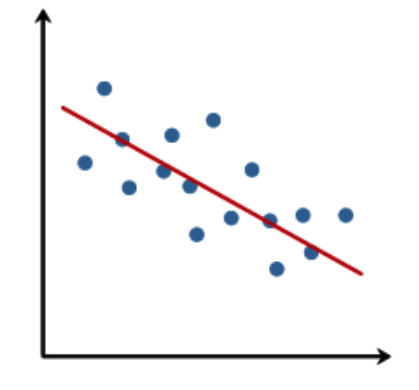
\includegraphics[width=0.8\linewidth]{figures-gradient/linear_regression.png}
\end{figure}
\end{minipage}
\end{frame}

\begin{frame}{Gradient descent for linear regression}
A typical linear regression model:
\begin{itemize}
	\item $\x \in \mathbb{R}^{D\times 1}$: input features; $y \in \mathbb{R}$: output value
	\item Model and loss:
	$$f(\x, \mparam ) = \x^\top \mparam, \quad y = f(\x, \mparam ) + \epsilon, \ \epsilon \sim \mathcal{N}(0, \sigma^2)$$
	$$L(\mparam ) = \frac{1}{2 \sigma^2} \sum_{n} (f(\x_n, \mparam ) - y_n)^2$$\pause
	\item Rewriting the loss in matrix form:
	$$L(\mparam ) = \frac{1}{2 \sigma^2} || \y - \X \mparam ||_2^2$$
\end{itemize}

\end{frame}

\begin{frame}{Gradient descent for linear regression}
Gradient descent to find $\mparam^*$:

Assume constant step-sizes $\gamma_t = \gamma$:
\begin{enumerate}
\item Define \emph{starting point} $\mparam_0$, set $t\gets 0$
\item Set $\mparam_{t+1} = \mparam_t - \gamma_t \nabla_{\mparam} L(\mparam_t)$, $t \leftarrow t+1$
\begin{equation*}
\begin{aligned}
\mparam_{t+1} &= \mparam_t - \gamma_t \nabla_{\mparam} L(\mparam_t) \\
&= \mparam_t - \gamma \frac{1}{\sigma^2}\X^\top(\X \mparam_t - \y) \\ \pause
&\textcolor{red}{= (\mathbf{I} - \frac{\gamma}{\sigma^2} \X^\top \X) \mparam_t + \frac{\gamma}{\sigma^2} \X^\top \y}
\end{aligned}
\end{equation*}
%
\item Repeat 1 until stopping criterion.
\end{enumerate}

\end{frame}

\begin{frame}{Gradient descent for linear regression}
Gradient descent to find $\mparam^*$:

Assume constant step-sizes $\gamma_t = \gamma$:
\begin{itemize}
\item GD returns the following iterative updates:
\begin{equation*}
\mparam_{t+1} = (\mathbf{I} - \frac{\gamma}{\sigma^2} \X^\top \X) \mparam_t + \frac{\gamma}{\sigma^2} \X^\top \y
\end{equation*}
%
\item We would like to figure out $\mparam_{t}$ as a function of $\mparam_0$ and $\gamma$! \\ (and also other hyper-parameters \& data)
\end{itemize}
\end{frame}

\begin{frame}{Gradient descent for linear regression}

Arithmetico-geometric sequence:

If a sequence $\{\mparam_0, \mparam_1, ..., \mparam_T \}$ is defined by
$$\mparam_{t+1} = \BB \mparam_t + \bm{c}, \quad t \geq 0,$$
Then we have
$$\mparam_{t+1} = \BA (\mparam_t + \bm{\beta}) - \bm{\beta}, \quad \text{for some } \BA, \bm{\beta}.$$ \pause

Let's work out what are $\BA$ and $\bm{\beta}$:
\begin{equation*}
\centering
\begin{aligned}
\mparam_{t+1} = &\mathbf{A}(\mparam_t + \bm{\beta}) - \bm{\beta} = \BB \mparam_t + \bm{c} \\
\Leftrightarrow \quad &\mathbf{A}\mparam_t + (\mathbf{A} - \mathbf{I}) \bm{\beta} = \BB \mparam_t + \bm{c} \\
\Leftrightarrow \quad &\BA = \BB, \quad \bm{\beta} = (\BB - \mathbf{I})^{-1} \bm{c}
\end{aligned}
\end{equation*}\pause
%
$$\Rightarrow \quad \mparam_{t+1} = \BB(\mparam_t + (\BB - \mathbf{I})^{-1} \bm{c} ) - (\BB - \mathbf{I})^{-1} \bm{c}$$
$$\Rightarrow \quad \mparam_t = \BB^t(\mparam_0 + (\BB - \mathbf{I})^{-1} \bm{c} ) - (\BB - \mathbf{I})^{-1} \bm{c}$$
\end{frame}


\begin{frame}{Gradient descent for linear regression}
Gradient descent to find $\mparam^*$:

Assume constant step-sizes $\gamma_t = \gamma$:
\begin{itemize}
\item GD returns the following iterative updates:
\begin{equation*}
\mparam_{t+1} = (\mathbf{I} - \frac{\gamma}{\sigma^2} \X^\top \X) \mparam_t + \frac{\gamma}{\sigma^2} \X^\top \y
\end{equation*}
%
\item Solving this iterative update returns: \pause
$$\mparam_{t} = (\mathbf{I} - \frac{\gamma}{\sigma^2} \X^\top \X)^t (\mparam_0 - \mparam^*) + \mparam^*, \quad \mparam^* = (\X^\top \X)^{-1} \X^\top \y$$
\item GD converges ($\mparam_t \rightarrow \mparam^*$) if $(\mathbf{I} - \frac{\gamma}{\sigma^2} \X^\top \X)^t (\mparam_0 - \mparam^*) \rightarrow \bm{0}$
\end{itemize}
\end{frame}


%\begin{frame}{Eigen decomposition: Indications}
%Indications of $\BA = \BQ \Lambda \BQ^{-1}$:
%\begin{itemize}
%\item If $\lambda$ is an eigenvalue of $\BA$, then $\lambda^t$ is an eigenvalue of $\BA^t$: \pause
%$$\BA^t = \BQ \Lambda \BQ^{-1} \BQ \Lambda \BQ^{-1} \cdot\cdot\cdot \BQ^{-1} \Lambda \BQ^{-1} = \BQ \Lambda^t \BQ^{-1},$$
%$$\Lambda^t = \text{diag}(\lambda_1^t, ..., \lambda_D^t)$$ \pause
%\item If $\lambda$ is an eigenvalue of $\BA$, then $\lambda + \alpha$ is an eigenvalue of $\BA + \alpha \mathbf{I}$: \pause
%$$\BA + \alpha \mathbf{I} = \BQ \Lambda \BQ^{-1} + \BQ \alpha \mathbf{I} \BQ^{-1} = \BQ (\Lambda + \alpha \mathbf{I}) \BQ^{-1}, $$
%$$\Lambda + \alpha \mathbf{I} = \text{diag}(\lambda_1 + \alpha, ..., \lambda_D + \alpha)$$ \pause
%\item Combine: If $\lambda$ is an eigenvalue of $\BA$, \\then $(\lambda + \alpha)^t$ is an eigenvalue of $(\BA + \alpha \mathbf{I})^t$
%\end{itemize}
%
%\end{frame}


%\begin{frame}{Eigen decomposition: Indications}
%Indications of $\BA = \BQ \Lambda \BQ^{-1}$: Assume $\BA$ is symmetric
%\begin{itemize}
%\item Consider the following \alert{Rayleigh quotient}
%$$R(\BA, \x) = \frac{\x^\top \BA \x}{|| \x ||_2^2}, \quad || \x ||_2^2 = \x^\top \x$$
%\item We can show that
%$$\lambda_{min}(\BA) \leq R(\BA, \x) \leq \lambda_{max}(\BA)$$
%$$\Rightarrow \quad \lambda_{min}(\BA) || \x ||_2^2 \leq \x^\top \BA \x \leq \lambda_{max}(\BA) || \x ||_2^2$$
%\end{itemize}
%
%\end{frame}

%\begin{frame}
%(break)
%\end{frame}

%\begin{frame}{Eigen decomposition: Indications}
%Indications of $\BA = \BQ \Lambda \BQ^{-1}$: Assume $\BA$ is symmetric
%\begin{itemize}
%\item Consider the following \alert{Rayleigh quotient}
%$$R(\BA, \x) = \frac{\x^\top \BA \x}{|| \x ||_2^2}, \quad || \x ||_2^2 = \x^\top \x$$
%\item We can show: $\lambda_{min}(\BA) \leq R(\BA, \x) \leq \lambda_{max}(\BA)$\\
%$\Rightarrow \quad \lambda_{min}(\BA) || \x ||_2^2 \leq \x^\top \BA \x \leq \lambda_{max}(\BA) || \x ||_2^2$
%\end{itemize}
%\vspace{12em}
%\end{frame}

%%%%%% analyse convergence %%%%%%%

\begin{frame}{Convergence of GD for linear regression}
Gradient descent with constant step-size to find $\mparam^*$:
$$\mparam_{t} = (\mathbf{I} - \frac{\gamma}{\sigma^2} \X^\top \X)^t (\mparam_0 - \mparam^*) + \mparam^*, \quad \mparam^* = (\X^\top \X)^{-1} \X^\top \y$$


\begin{itemize}
\item The $\ell_2$ distance between $\mparam_t$ and $\mparam^*$:
\begin{equation*}
\begin{aligned}
|| \mparam_t - \mparam^* ||_2^2 &= || (\mathbf{I} - \frac{\gamma}{\sigma^2} \X^\top \X)^t (\mparam_0 - \mparam^*) ||_2^2 \\
&= | (\mparam_0 - \mparam^*)^\top (\mathbf{I} - \frac{\gamma}{\sigma^2} \X^\top \X)^{2t} (\mparam_0 - \mparam^*) |
\end{aligned}
\end{equation*}
%\only<1>{
%\item Notice that a Rayleigh quotient satisfies $\lambda_{min}(\BA) || \x ||_2^2 \leq \x^\top \BA \x \leq \lambda_{max}(\BA) || \x ||_2^2$
%\item Also if $\lambda$ is an eigenvalue of $\BA$, then $\lambda^{t}$ is an eigenvalue of $\BA^t$
%}
%
\visible<2->{
\item Fact: $\lambda_{min}(\BA) || \x ||_2^2 \leq \x^\top \BA \x \leq \lambda_{max}(\BA) || \x ||_2^2$:
\only<2>{
$$|| \mparam_t - \mparam^* ||_2^2 \geq \lambda_{min}((\mathbf{I} - \frac{\gamma}{\sigma^2} \X^\top \X)^{2t}) || \mparam_0 - \mparam^* ||_2^2$$
$$|| \mparam_t - \mparam^* ||_2^2 \leq \lambda_{max}((\mathbf{I} - \frac{\gamma}{\sigma^2} \X^\top \X)^{2t}) || \mparam_0 - \mparam^* ||_2^2$$
}
\only<3>{
$$|| \mparam_t - \mparam^* ||_2^2 \geq \textcolor{red}{\lambda_{min}((\mathbf{I} - \frac{\gamma}{\sigma^2} \X^\top \X)^{2})^t} || \mparam_0 - \mparam^* ||_2^2$$
$$|| \mparam_t - \mparam^* ||_2^2 \leq \textcolor{red}{\lambda_{max}((\mathbf{I} - \frac{\gamma}{\sigma^2} \X^\top \X)^{2})^t} || \mparam_0 - \mparam^* ||_2^2$$
}
}
\end{itemize}

\end{frame}

\begin{frame}{Convergence of GD for linear regression}
Gradient descent with constant step-size to find $\mparam^*$:
$$\lambda_{min}^{t} || \mparam_0 - \mparam^* ||_2^2 \leq || \mparam_t - \mparam^* ||_2^2 \leq \lambda_{max}^{t} || \mparam_0 - \mparam^* ||_2^2$$
$$\lambda_{min} := \lambda_{min}((\mathbf{I} - \frac{\gamma}{\sigma^2} \X^\top \X)^2) \geq 0, \quad \lambda_{max} := \lambda_{max}((\mathbf{I} - \frac{\gamma}{\sigma^2} \X^\top \X)^2)$$ \pause

Convergence properties in difference cases:
\begin{enumerate}
\item $\lambda_{max} < 1$: always converge
\item $\lambda_{min} \geq 1$: always diverge
\item $\lambda_{min} < 1$ but $\lambda_{max} \geq 1$: convergence depending on $\mparam_0$
\end{enumerate}

\end{frame}


\begin{frame}{Convergence of GD for linear regression}
Gradient descent with constant step-size to find $\mparam^*$:
$$\lambda_{min}^{t} || \mparam_0 - \mparam^* ||_2^2 \leq || \mparam_t - \mparam^* ||_2^2 \leq \lambda_{max}^{t} || \mparam_0 - \mparam^* ||_2^2$$
$$\lambda_{min} := \lambda_{min}((\mathbf{I} - \frac{\gamma}{\sigma^2} \X^\top \X)^2) \geq 0, \quad \lambda_{max} := \lambda_{max}((\mathbf{I} - \frac{\gamma}{\sigma^2} \X^\top \X)^2)$$

Deriving the eigenvalues $\lambda_{min}, \lambda_{max}$: \pause
\begin{itemize}
\item If $\lambda$ is an eigenvalue of $\mathbf{I} - \frac{\gamma}{\sigma^2} \X^\top \X$, \\then $\lambda^2$ is an eigenvalue of $(\mathbf{I} - \frac{\gamma}{\sigma^2} \X^\top \X)^2$ \pause
\item If $\lambda$ is an eigenvalue of $\X^\top \X$, \\
then $1 - \frac{\gamma \lambda}{\sigma^2}$ is an eigenvalue of $\mathbf{I} - \frac{\gamma}{\sigma^2} \X^\top \X$:
$$\X^\top \X \bm{q} = \lambda \bm{q} \quad \Leftrightarrow \quad (\mathbf{I} - \frac{\gamma}{\sigma^2} \X^\top \X) \bm{q} = (1 - \frac{\gamma \lambda}{\sigma^2}) \bm{q}$$
\end{itemize}

\end{frame}

\begin{frame}{Convergence of GD for linear regression}
Gradient descent with constant step-size to find $\mparam^*$:
$$\lambda_{min}^{t} || \mparam_0 - \mparam^* ||_2^2 \leq || \mparam_t - \mparam^* ||_2^2 \leq \lambda_{max}^{t} || \mparam_0 - \mparam^* ||_2^2$$
$$\lambda_{min} := \lambda_{min}((\mathbf{I} - \frac{\gamma}{\sigma^2} \X^\top \X)^2) \geq 0, \quad \lambda_{max} := \lambda_{max}((\mathbf{I} - \frac{\gamma}{\sigma^2} \X^\top \X)^2)$$

\begin{itemize}
\item If $\lambda$ is an eigenvalue of $\X^\top \X$, \\
then $(1 - \frac{\gamma \lambda}{\sigma^2})^2$ is an eigenvalue of $(\mathbf{I} - \frac{\gamma}{\sigma^2} \X^\top \X)^2$ \pause
\item $\X^\top \X$ is positive semi-definite $\Rightarrow \lambda \geq 0$ \pause
\item Ensuring convergence: we want $\lambda_{max} = \max (1 - \frac{\gamma \lambda}{\sigma^2})^2 < 1$
$$\Rightarrow \gamma < \frac{2 \sigma^2}{\lambda_{max}(\X^\top \X)} $$
\end{itemize}

\end{frame}


\begin{frame}{Choosing step-size for linear regression}

To ensure convergence at \alert{any} initialisation: $\gamma < 2 \sigma^2 / \lambda_{max}(\X^\top \X)$

\alert{Q:} Can we use larger step-sizes?\\ \pause
\alert{A:} Yes and No.

\begin{enumerate}
\item You choose a step-size $\gamma \geq 2 \sigma^2 / \lambda_{min}(\X^\top \X) \quad \Rightarrow$ diverge  \pause
\item You choose a step-size $\gamma \in [ \frac{2\sigma^2}{\lambda_{max}(\X^\top \X)},  \frac{2\sigma^2}{\lambda_{min}(\X^\top \X)} ) \quad \Rightarrow$ good luck
\begin{itemize}
	\item Convergence result may be sensitive to initialisation $\bm{\theta}_0$
\end{itemize}
\end{enumerate}

\end{frame}


\begin{frame}{Choosing step-size for linear regression}

To ensure convergence at \alert{any} initialisation: $\gamma < 2 \sigma^2 / \lambda_{max}(\X^\top \X)$

If you want to test your luck: choose $\gamma \in [ \frac{2\sigma^2}{\lambda_{max}(\X^\top \X)},  \frac{2\sigma^2}{\lambda_{min}(\X^\top \X)} )$

Is my choice of $\gamma$ robust to initialisation of $\mparam_0$? \pause
\begin{itemize}
\item Depending on the \alert{condition number}:
$$ \kappa(\X^\top \X) := \frac{\lambda_{max}(\X^\top \X)}{\lambda_{min}(\X^\top \X)} $$
\end{itemize}
\vspace{-0.5em}

\hspace{7em}
\begin{minipage}{0.18\linewidth}
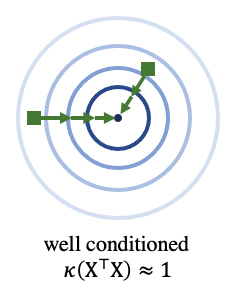
\includegraphics[width=1\linewidth]{figures-gradient/well_conditioned.png}
\end{minipage}
\hspace{3em}
\begin{minipage}{0.25\linewidth}
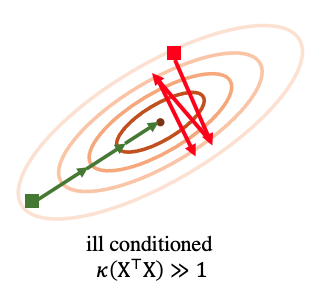
\includegraphics[width=1\linewidth]{figures-gradient/ill_conditioned.png}
\end{minipage}

\begin{itemize}
\item Need careful choice of step-sizes if the loss is ``very stretched'' \pause
\item Note: $\kappa(\X^\top \X) = \kappa(\X)^2 = \frac{\sigma_{max}(\X)}{\sigma_{min}(\X)}$
\end{itemize}

\end{frame}

\begin{frame}{Choosing step-size: general case}

In general the loss function is non-quadratic nor convex:
\only<1>{
  \begin{figure}
    \centering
    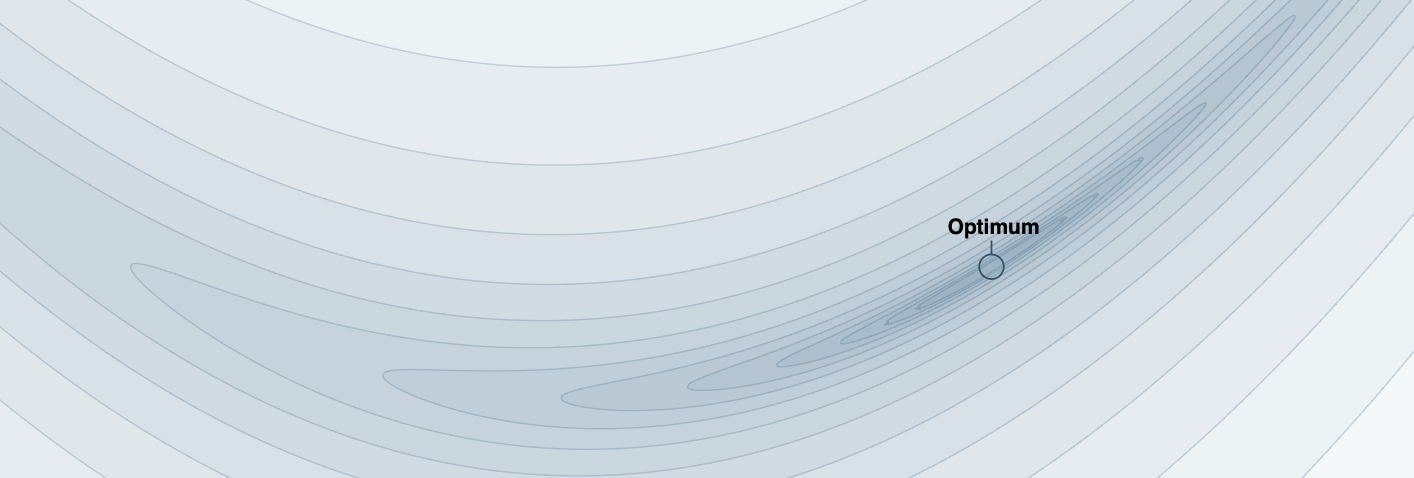
\includegraphics[width = 1.0\hsize]{figures-gradient/loss_landscape_conditioning0.png}
  \end{figure}}
\only<2>{
  \begin{figure}
    \centering
    
\includegraphics[width = 1.0\hsize]{figures-gradient/loss_landscape_conditioning1.png}
  \end{figure}}
  
\visible<2>{
Local quadratic approximation when $\mparam_t \approx \mparam^*$:
\begin{itemize}
\item locally approximate $L(\mparam_t) \approx L(\mparam^*) + \frac{1}{2} (\mparam_t - \mparam^*)^\top \nabla^2 L(\mparam^*) (\mparam_t - \mparam^*)$ \\
(in linear regression $\nabla^2 L(\mparam) \ \propto \ \X^\top \X$)
\item $\kappa(\nabla^2 L )$ can tell whether the loss is ``locally stretched''
\end{itemize}
}

\hfill \tiny{\url{https://distill.pub/2017/momentum/}}
\end{frame}

\begin{frame}{Choosing step-size: general case}
Let's see what happens for different step-sizes.
\only<1>{
  \begin{figure}
    \centering
    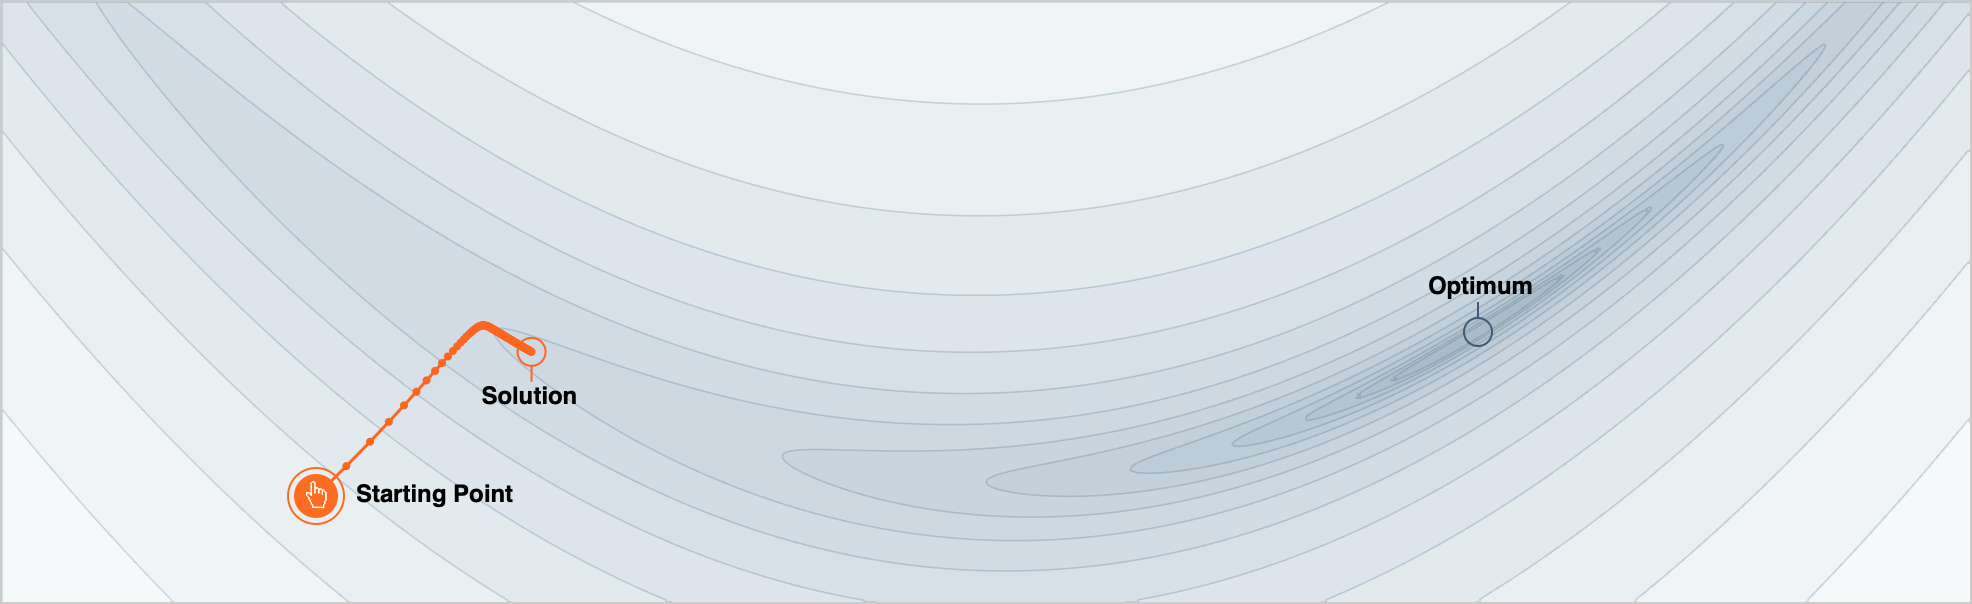
\includegraphics[width = 1.0\hsize]{./figures-gradient/gd-step-1.png}
  \end{figure}}
\only<2>{
  \begin{figure}
    \centering
    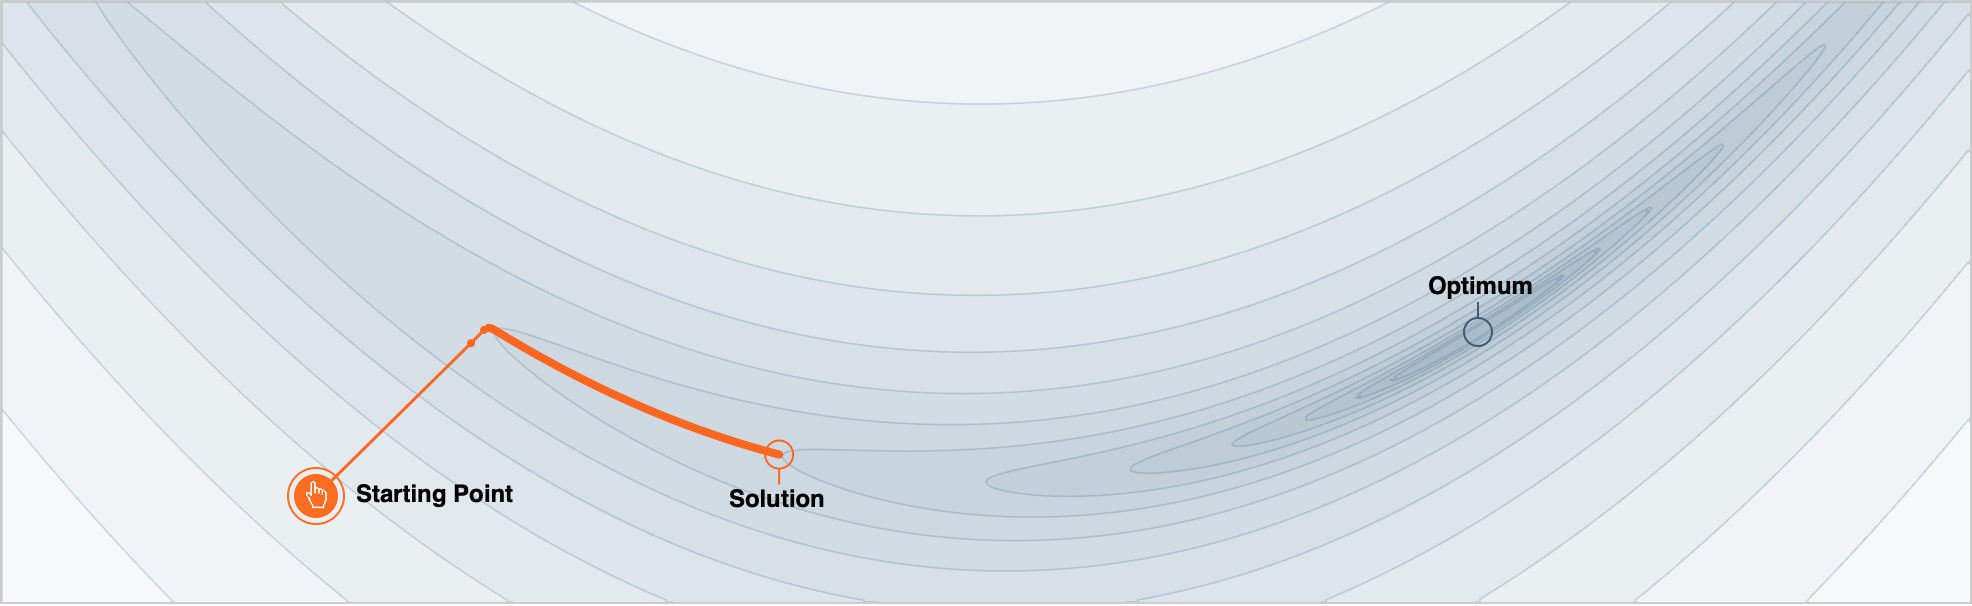
\includegraphics[width = 1.0\hsize]{./figures-gradient/gd-step-2.png}
  \end{figure}}
\only<3>{
  \begin{figure}
    \centering
    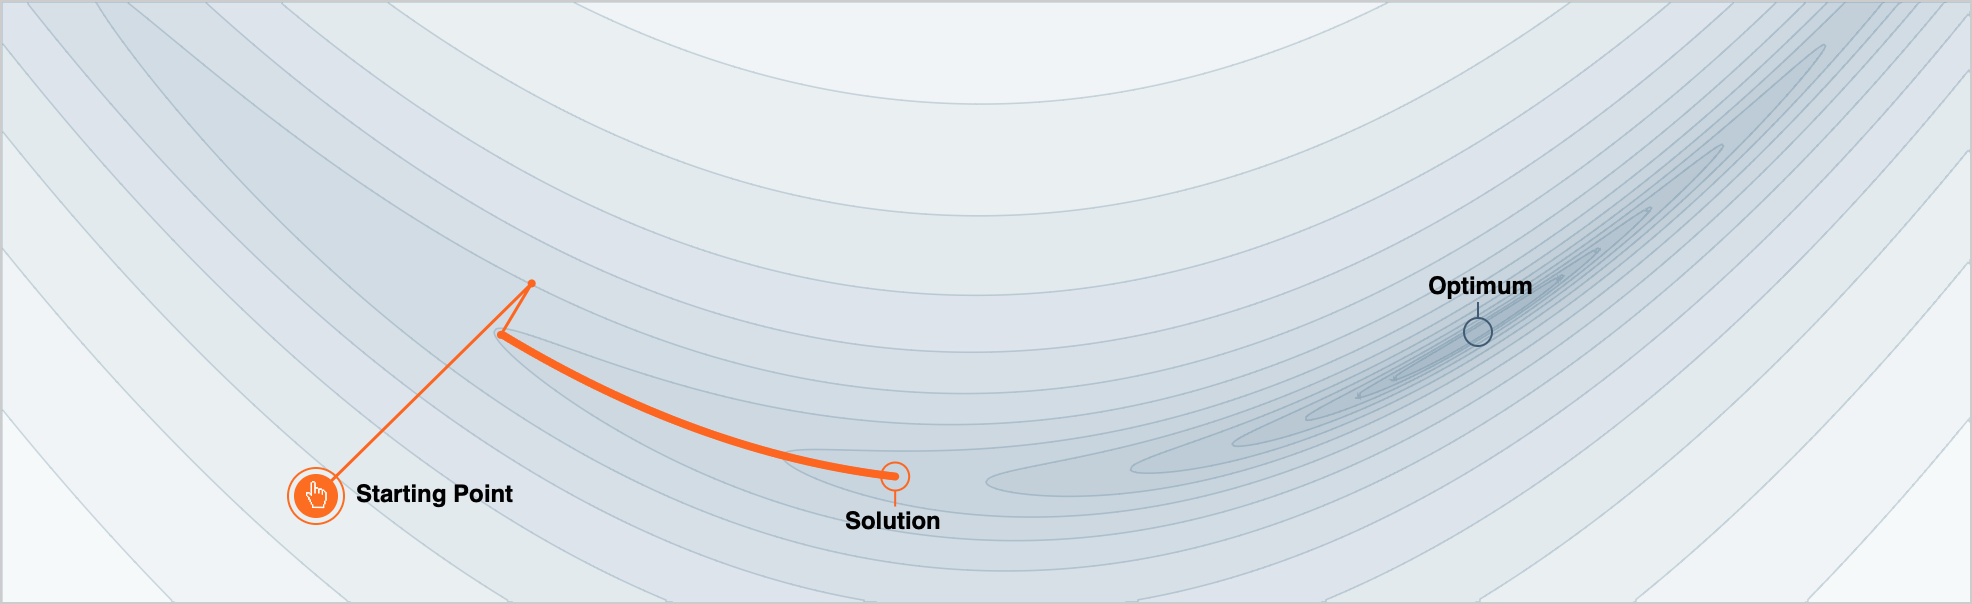
\includegraphics[width = 1.0\hsize]{./figures-gradient/gd-step-3.png}
  \end{figure}}
\only<4>{
  \begin{figure}
    \centering
    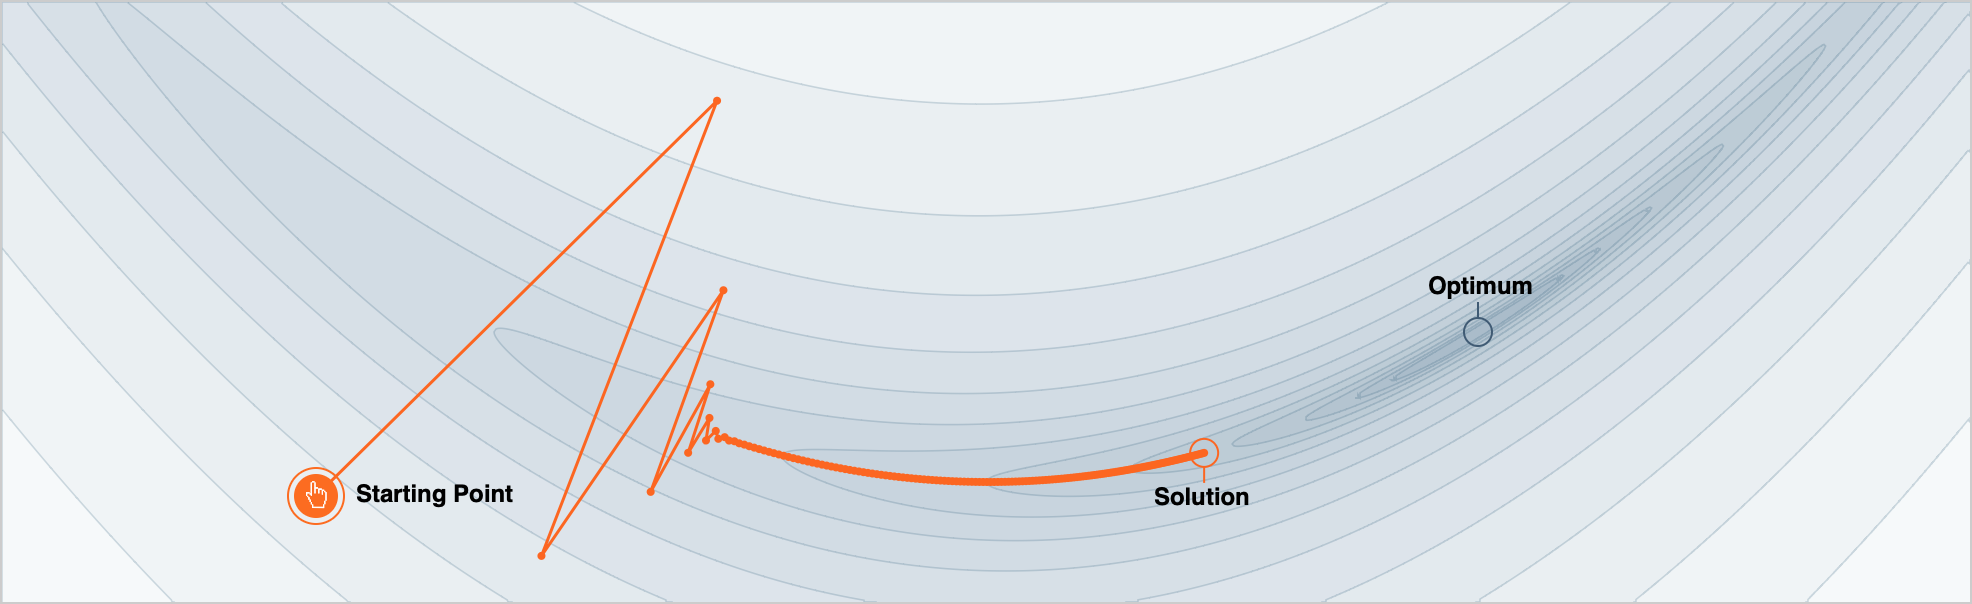
\includegraphics[width = 1.0\hsize]{./figures-gradient/gd-step-4.png}
  \end{figure}}
\only<5>{
  \begin{figure}
    \centering
    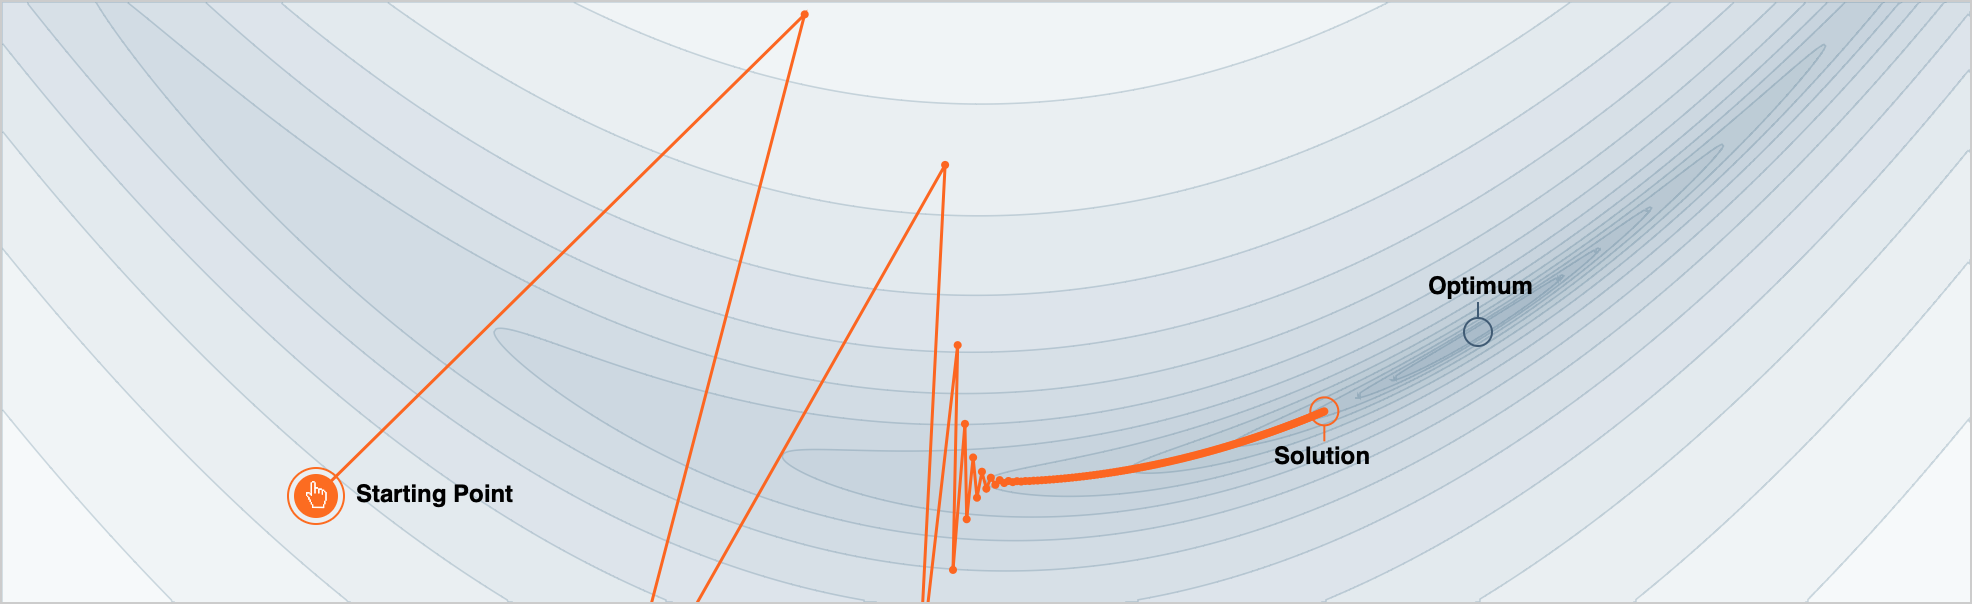
\includegraphics[width = 1.0\hsize]{./figures-gradient/gd-step-5.png}
  \end{figure}}
\only<6>{
  \begin{figure}
    \centering
    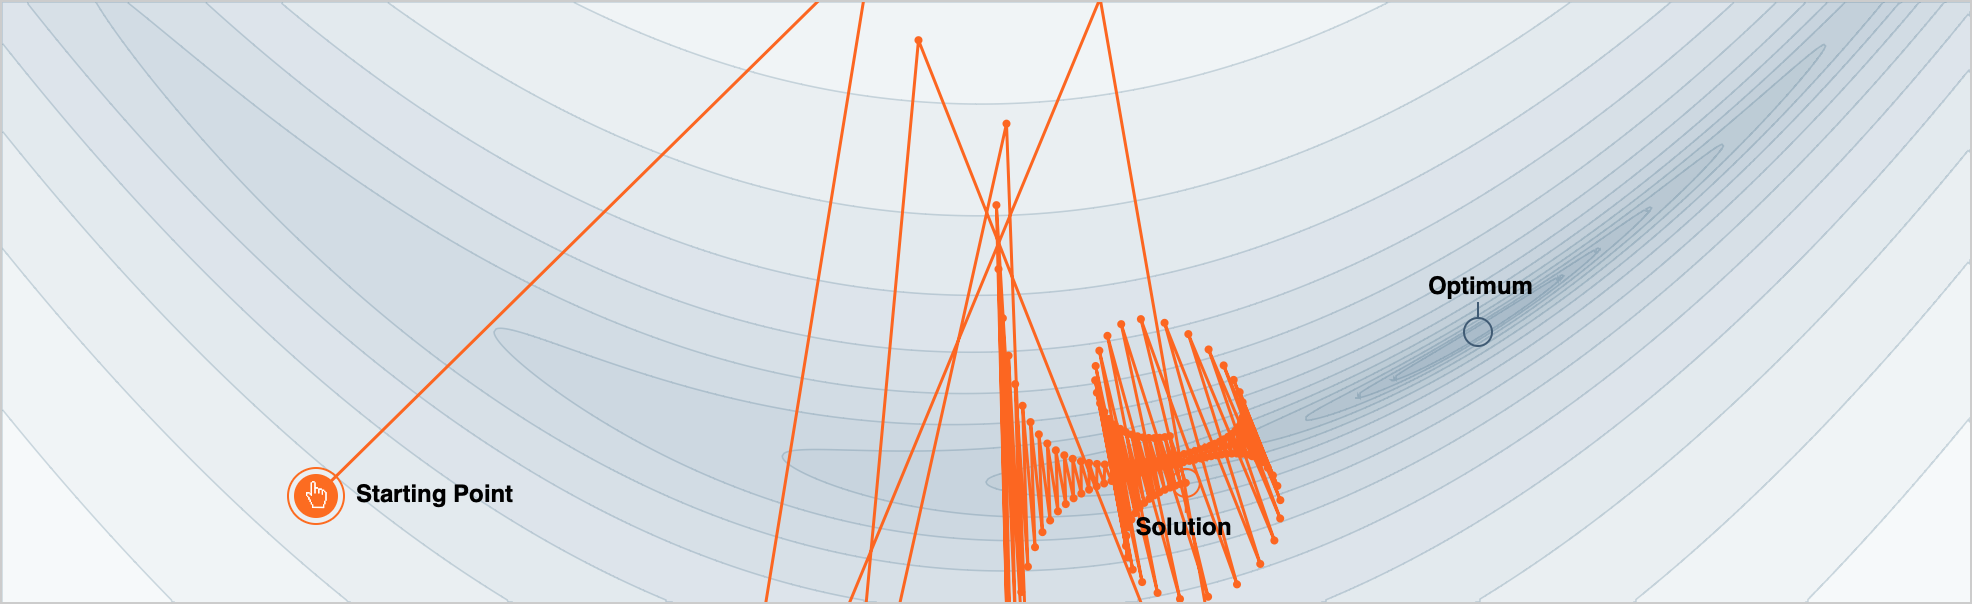
\includegraphics[width = 1.0\hsize]{./figures-gradient/gd-step-6.png}
  \end{figure}}
Image shows:
\begin{itemize}
\item Path of $\mparam_t$ from Gradient Descent
\item Constant step size $\gamma_t = \gamma$
\end{itemize}

\hfill \tiny{\url{https://distill.pub/2017/momentum/}}
\end{frame}

\begin{frame}{Choosing step-size: summary}

Summary on choosing step size:
\begin{itemize}
\item too small: slow convergence
\item too large: divergence
\item just right: depends on problem (often: trial and error)
\end{itemize}\pause

\begin{center}
Rule of thumb: \\ 
Start from a relatively large step size, \\
decrease step size as getting closer to a (local) optimum.
\end{center}
\end{frame}

\begin{frame}{Exercises}

Finish relevant exercises in the exercise sheet
\begin{itemize}
	\item You should be able to analyse more advanced gradient-based optimisation methods for linear regression
\end{itemize}

\vspace{1em}

Next lecture: multivariate probability

Pre-requisite knowledge: univariate probability

\end{frame}

\end{document}
%%% Local Variables: 
%%% mode: latex
%%% TeX-master: t
%%% End: 
